\documentclass{article}
\usepackage{packages}

\begin{document}

\section*{Push-forward and pull-back}

\subsubsection*{Pull-back of a function}
\begin{figure}[h]
    \centering
    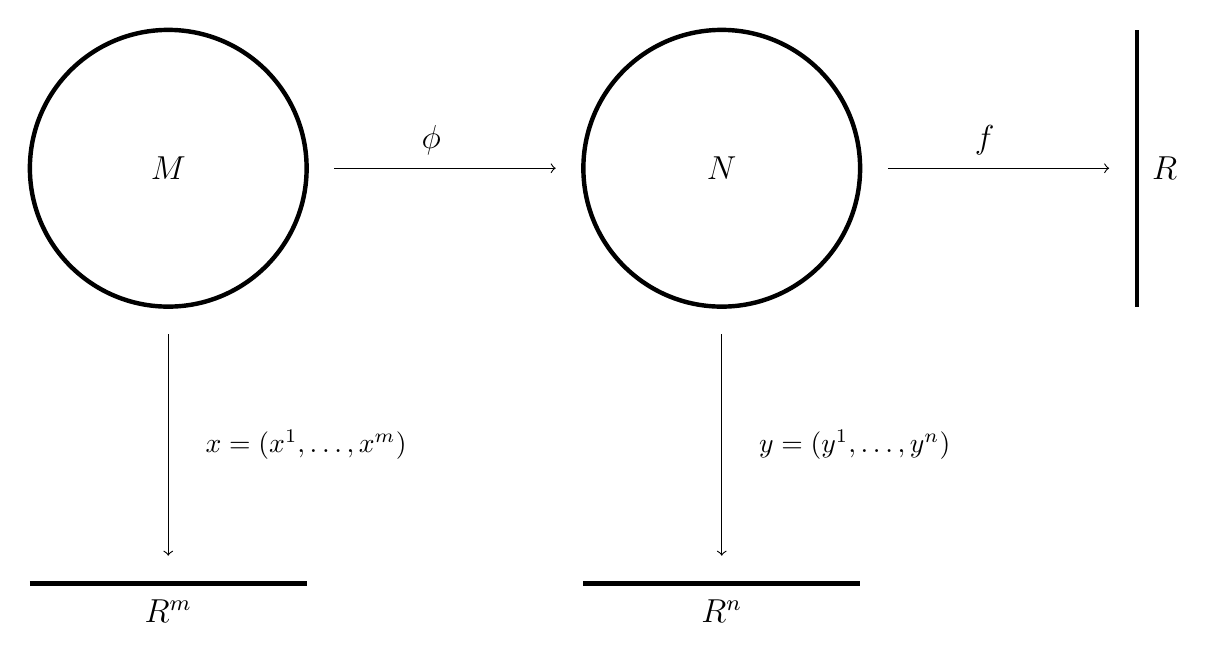
\begin{tikzpicture}
        \draw[black, ultra thick] (0,0) circle (50pt);
        \node[] at (0,0) {\bfseries\large $M$};

        \draw[->] (60pt,0) -- (140pt,0);
        \node[] at (95pt,10pt) {\large $\phi$};

        \draw[black, ultra thick] (200pt,0) circle (50pt);
        \node[] at (200pt,0) {\bfseries\large $N$};

        \draw[->] (260pt,0) -- (340pt,0);
        \node[] at (295pt,10pt) {\large $f$};

        \draw[black, ultra thick] (350pt,-50pt) -- (350pt,50pt);
        \node[] at (360pt,0) {\large $\mathbb{R}$};

        \draw[->] (0,-60pt) -- (0,-140pt);
        \node[anchor=west] at (10pt,-100pt) {$x = (x^1, \dots, x^m)$}; 
        \draw[black, ultra thick] (-50pt,-150pt) -- (50pt,-150pt);
        \node[] at (0,-160pt) {\large $\mathbb{R}^m$};

        \draw[->] (200pt,-60pt) -- (200pt,-140pt);
        \node[anchor=west] at (210pt,-100pt) {$y = (y^1, \dots, y^n)$}; 
        \draw[black, ultra thick] (150pt,-150pt) -- (250pt,-150pt);
        \node[] at (200pt,-160pt) {\large $\mathbb{R}^n$};

    \end{tikzpicture}
\end{figure}
Let us consider two manifolds M and N, respectively m-dimensional and n-dimensional. \\
Let us then consider a mapping between the two manifolds $\phi : M \to N$ and a function $f: N \to \mathbb{R}$. \\
Let us now consider a vector $V \in T_pM$ where $p \in M$. The vector $V$ is "a derivation" operator acting on smooth functions on M. Given a set of coordinate functions $x = (x^1, \dots, x^m)$ on $M$, a coordinate representation
of $V$ is $V = V^{\mu} \frac{\partial}{\partial x^\mu}$. \\
By definition the differential operator $V$ can act only on functions on $M$. Thus it is possible to make it act on $f$ by \emph{pulling $f$ back} to M trough $\phi$. \\
Indeed the application $f \circ \phi$ maps a point of $M$ in $\mathbb{R}$, hence such a function can be differentiated by $X$. The operation of \emph{pulling $f$ back} to $M$ is called \emph{pull-back} of $f$. 
More precisely, the pull-back of any smooth function on $N$ is a function
\begin{equation*}
    \phi^* : \mathcal{S}(N) \to \mathcal{S}(M)
\end{equation*}
where $\mathcal{S}(A)$ indicates the set of smooth functions acting on $A$, and its action is defined as
\begin{equation*}
    V(\phi^* f)_p = V(f \circ \phi)
\end{equation*}
where the subscript $p$ means that it acts on $M$ (from now on this will be omitted considering it implicit).
In coordinates $f(\phi(p)) = f(\phi(x^{-1}(\mathbf{x}))) \Rightarrow f = f(\mathbf{x})$ where $\mathbf{x} \in \mathbb{R}^m$. Hence
\begin{equation*}
    V(\phi_*f) = V^\mu \frac{\partial f(\mathbf{x})}{\partial x^\mu}
\end{equation*}

\subsubsection*{Push-forward of a vector}
The same result above can also be seen as the result of the action of another operator, namely the \emph{push-forward}, which we denote as $\phi_*$, whose
role is to \emph{push $V$ forward} to $N$, so that $\phi_* V \in T_{\phi(p)} N$ and its action on a function $f: N \to \mathbb{R}$ is defined by requesting that
\begin{equation}
    (\phi_* V)_{\phi(p)} \, f = V(\phi^* f)_p = V(f \circ \phi)
    \label{eq:push_forward_vector}
\end{equation}
where, again, the subscript $\phi_(p)$ indicates that $\phi_* V$ is a vector in $T_{\phi(p)}N$ (and again from later on the subscript will be dropped and considered implicit). \\
What we did previousle was extending $f$ to $M$ and working in the manifold $M$. Here, instead, we are extending $V$ to $N$ and working on $N$. \\
Now let us introduce the charts $x = (x^1, \dots, x^m)$ in $M$ and $ y = (y^1, \dots, y^m)$ in $N$.
A coordinate representation of $V$ is $V = V^\mu \frac{\partial}{\partial x^\mu}$. \\
Since $\phi_* V$ is a vector in $T_{\phi(p)} N$ a coordinate representation is 
$\phi_* V = (\phi_*V)^\mu\frac{\partial}{\partial y^\mu}$. \\
To get each component $(\phi_* V)^\alpha$ we must make $\phi_* V$ act on each coordinate $y^\alpha$ so that
\begin{equation*}
    (\phi_* V)y^\alpha = \left((\phi_*V)^\mu\frac{\partial}{\partial y^\mu}\right) y^\alpha = (\phi_*V)^\mu  = (\phi_*V)^\mu\frac{\partial y^\alpha}{\partial y^\mu} = (\phi_*V)^\mu \delta_\mu^\alpha = (\phi_* V)^\alpha
\end{equation*}
In other words we extraced the components $\alpha$ of the vector $\phi_* V \in T_{\phi(p)}N$. \\
By using the definition given by \ref{eq:push_forward_vector} and the coordinate representation of $V$
\begin{equation}\begin{gathered}
    (\phi_* V)^\alpha = (\phi_* V) \, y^\alpha = V (y^\alpha \circ \phi) = V^\mu \frac{\partial}{\partial x^\mu}(y^\alpha \circ \phi) = \\
    = V^\mu \frac{\partial}{\partial x^\mu}(y^\alpha(\phi(p))) = V^\mu \frac{\partial}{\partial x^\mu}(y^\alpha(\phi(x^{-1}(\textbf{x}))))
    \label{eq:push_forward_coordinates}
\end{gathered}\end{equation}
where $\textbf{x} = x(p) = (x^1, \dots, x^m) \in \mathbf{R}^m$. \\
The last member of equation \ref{eq:push_forward_vector} tells us that we can consider $y^\alpha$ as a function of $\mathbf{x}$. \\
Hence $y^\alpha = y^{\alpha}(\mathbf{x})$. Finally, equation \ref{eq:push_forward_coordinates} reduces to 
\begin{equation*}
    (\phi_* V)^\alpha = V^\mu \frac{\partial y^\alpha}{\partial x^\mu}
\end{equation*}
Sounds familiar? The function $\phi_*$ acts on $V$ as a jacobian matrix \footnote{Note that since we are working on a manifold, this holds only locally! And this is why the push-forward is the generalization of the jacobian matrix. The two things coincide when we work in $\mathbb{R}^n$.}. \\
Since $\phi_* V \in T_{\phi(p)}N$ we can make it act on a differential form $\omega \in T_{\phi(p)}^*N$.
\begin{gather*}
    \phi_* V = (\phi_*V)^\mu \frac{\partial}{\partial y^\mu} \\
    \omega = \omega^\mu dy^\mu \\
    (\phi_* V)(\omega) = \omega(\phi_*V) = \left\langle \phi_*V, \omega \right\rangle = V^\mu \omega^\nu \left\langle\frac{\partial}{\partial y^\mu}, dy^\nu \right\rangle = V^\mu \omega^\mu
\end{gather*}

\subsubsection*{Pull-back of a differential form}
The result we have just obtained can be seen in another way. Indeed, instead of \emph{pushing V forward} to $N$ (working on $N$), we can \emph{pull $\omega$ back} to $V$ (working on $N$). More precisely
we can introduce a new differential form $\phi^*\omega \in T_p^* M$ by requesting that
\begin{equation*}
    \left\langle \phi_* V, \omega \right\rangle = \left\langle V, \phi^*\omega \right\rangle
\end{equation*}
The map $\phi^* : T_{\phi(p)}^* N \to T_p^* M$ is called \emph{pull-back} of $\omega$. \\
This nicely shows that the pull-back $\phi^*$ and the push-forward $\phi_*$ are dual functions one to the other.

\subsubsection*{Integral curves and flows}
Let us consider a vector field $\chi$ on $M$, that is a a function that assigns a vector to each point of the manifold
\begin{gather*}
    \chi: M \to TM \\
    p \to v \in T_pM
\end{gather*}
Given a set of coordinates in a neighbourhood of a point $p \in M$, the vector defined by $\chi$ at the point $p$ is $\chi(p) = X^\mu(x(p)) \frac{\partial}{\partial x^\mu}_{|_p}$. \\
The vector field $\chi$ defines a curve $\sigma$ (namely the \emph{integral curve} of $\chi$) trough the relation
\begin{equation}
    \frac{d}{dt} \sigma(t) = \chi(\sigma(t))
    \label{eq:integral_curve}
\end{equation}
which in coordinates reads
\begin{equation*}
    \frac{d}{dt}x^\mu(\sigma(t)) = X^\mu(x(\sigma(t))) \qquad \mu = 1, \dots, m
\end{equation*}
We will mean this last equation when we write
\begin{equation*}
    \frac{d}{dt}\sigma^\mu(t) = X^\mu(\sigma(t))
\end{equation*}
Equation \ref{eq:integral_curve} means that the integral curve of a vector field $\chi$ is the one whose tanget vector to $\sigma$
at each point $p \in M$ is the vector given by $\chi(p)$. The general solution to the ODE is a family of functions. One can identify 
a particular solution by specifying a the value of the curve at a given point, e.g. $\sigma(t=0) = p \in M$. We will indicate such a particular solution 
as $\sigma(t, p)$. The function $\sigma(t, p)$ can be also seen as a function of the point in the manifold $p$
\begin{equation*}
    \sigma_t(p) : M \to M
\end{equation*}
We call such a function \emph{flow} generated by $\chi$.

\subsubsection*{Lie derivative}
\end{document}